\documentclass[12pt,a4paper]{article}

\usepackage[utf8]{inputenc}
\usepackage{graphicx}
\usepackage{float}

\begin{document}

\title{MI-PAA 2015 2.ukol}
\author{Tomas Nesrovnal\\nesrotom@fit.cvut.cz}
\date{\today}
\maketitle

\section{Specifikace ulohy}
Problem 0-1 batohu.

\section{Rozbor moznych variant reseni}
Ulohu muzu resit hrubou silou. Ziskam tam presny vysledek, ale vypocet bude
pomaly. Dalsim resenim je pouzit heuristiku, jejiz vyledek nebude nejlepsi mozny
ale vypocet probehne rychle.

\section{Ramcovy popis postupu reseni}
\subsection{Hruba sila}
Zkusim vsechny moznosti a vyberu tu nejlepsi.

\subsection{Heuristika}
Vkladam do bahothu nejlepsi predmety s pomerem cena/vaha, dokud
mi jeste staci kapacita.

\section{Popis kostry algoritmu}
\subsection{Hruba sila}
Vytvorim pole, ktere udava ktery predmet je v batohu. Rekurzivne zkousim
vsechny moznosti (zavolam rekurzi bez prvku, pak prvek pridam a zavolam rekurzi znovu).
Ulozim si nejlepsi reseni.

Druha varianta obsahuje vylepseni: Pokud ve stromu reseni narazim na to, ze se do batohu uz vic nevejde, vetev zariznu.

\subsection{Heuristika}
Seradim si pole s predmety podle pomeru cena/vaha (nebo jine varianty, viz grafy). Cele pole sestupne prochazim a pokud se tam predmet vejde, tak ho tam vlozim.

\section{Namerene vysledky}

\subsection{Spravnost vysledku}
Pomoci skriptu byla overena spravnost vysledku (porovnanim s referencnim resenim). U method s nepresnym vysledem byla zaznamenana maximalni a relativni chyba.

\subsection{Na cem bylo mereno}
Intel(R) Core(TM) i3-2328M Processor (3M Cache, 2.20 GHz), gcc 4.9.2 (-Ofast), OS GNU/Linux Lubuntu 14.04 64bit

\section{Branch and Bound}
Orezaval jsem ze shora i z dola. Pred tim jsem pole seradil jako v heuristice, aby bylo orezavani efektivnejsi.

\section{Dynamicke programovani}
Implementoval jsem dva zpusoby dymanickeho programovani. Jeden zpusob plnil tabulku od spoda nahoru (dva cykly v sobe).
Druhy resil odshora dolu (rekurze). Obe reseni vracely spravne vysledky, ale prvni zpusob byl mnohem rychlejsi.

Obe tyto reseni meli dekompozici podle vahy.

\section{FPTAS}
FPTAS je podobny heuristice. Nejdriv ale spocitam maximalni chybu a podle toho a podle nastavene mozne chyby epsilon preskaluji vstupni data. Pro chybu eps=0 byly tedy vysledky spravne, stejne jako u dynamickeho programovani.

Slozitost FPTAS se odviji od prednastavene chyby: $O(n^3 / epsilon)$
\section{Grafy}

Grafy predstavuji lineani funkce vytvorene z diskretnich hodnot.

\begin{figure}[H]
	\caption{Doba vypoctu}
 	\centerline{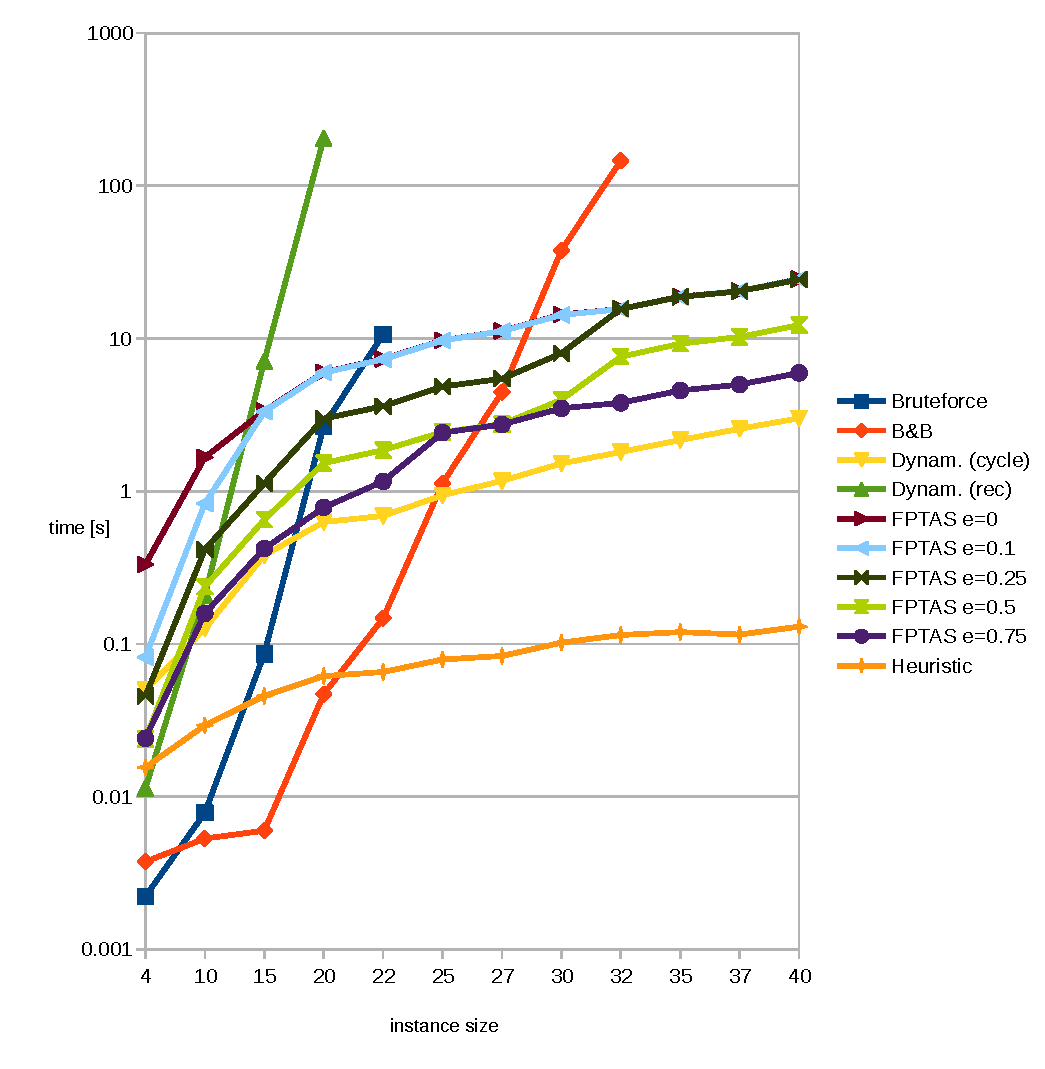
\includegraphics{./time_svg.pdf}}
\end{figure}

\begin{figure}[H]
	\caption{Maximalni a relativni chyba FPTAS}
 	\centerline{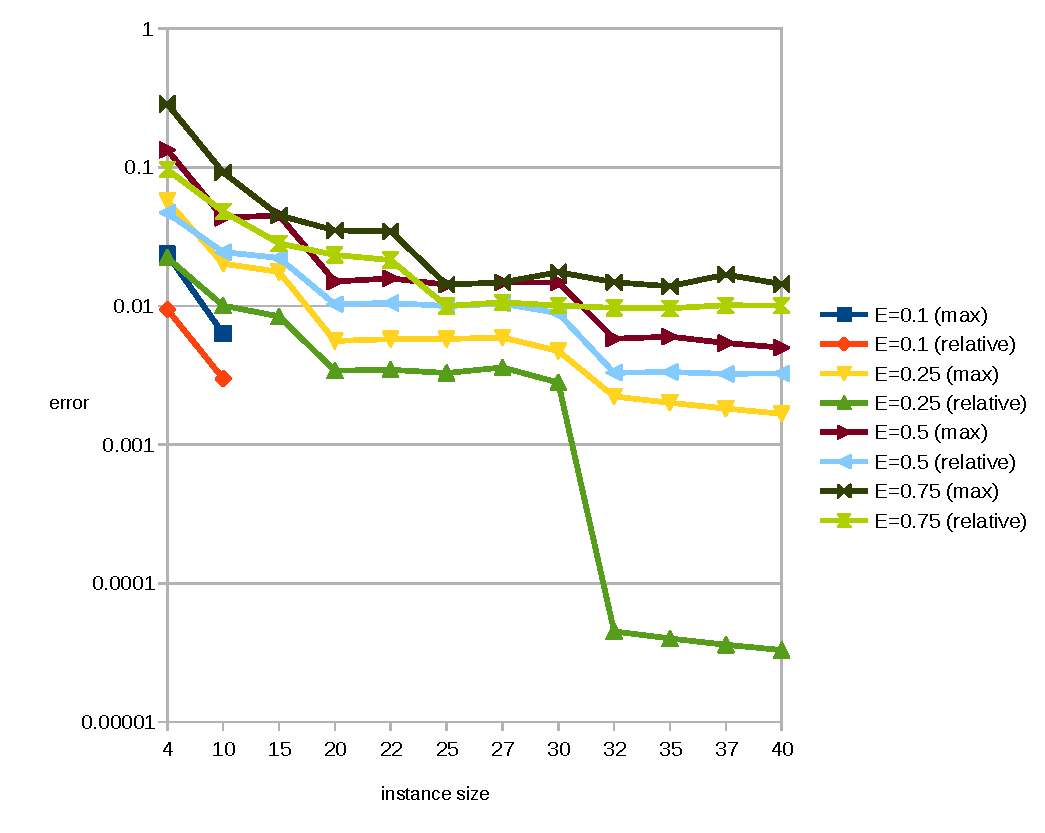
\includegraphics{./fptas_err.pdf}}
\end{figure}


\section{Zaver}
BB (optimalizovana v C) vyrazne pomohla, ale je hodne citliva na vstupni data. Ovsem asymptoticka slozitost zustava $O(2^n)$, protoze B\&B nezlepsi nejhorsi pripad.

Dynamicke programovani je lepsi (dle namerencyh udaju) provadet odspoda a je lepsi se vyhnout rekurzi.

FPTAS pocita s chybou, ale pri dobre zvolenem eps mame malou chybu a rychle reseni.

\subsection{Zhodnoceni}
Ocekavene vysledky potvrdilo mereni. Metoda B\&B se ukazala byt velice dobra pro maly pocet dat. FPTAS se ukazal byt rychly a relativne presny, ale klasicke dynamicke programovani bylo stale lepsi. Heuristika je stale nejrychlejsi, ale jeji vysledky jsou radove min presne nez u ostatnich metod.

%%%%%%%%%%%%%%%%%%%%%%%%%%%%%%%%%%%%%%%%%%%%%%%%%%%%%%%%
\end{document}
